In order to discriminate the shapes in our database, we describe each shape by a set of features.
We then use these features to compute a distance between a pair of shapes, which is relative to how dissimilar the two
shapes are.
This section discusses exactly what features we determine for each shape, how we calculate them, and how we
implemented these calculations.
An overview of all features that will be extracted for the 3D shapes can be seen in Table \ref{tab:features}.

\paragraph{Global descriptors}
Firstly, we compute some elementary descriptors for 3D objects, which are single values describing a shape from a
global perspective.
These features are the surface area, volume, diameter, eccentricity, and compactness of the shape, as well as three
ratios for comparisons between the shape and its bounding box or convex hull.

The bounding box of a 3D shape is the smallest rectangular box which fully encompasses the volume of the 3D shape.
We use the ratio between the volume of the shape  the volume of its bounding box, to moderately indicate how tightly
the shape fits in a rectangular box.

The convex hull of a 3D shape is the convex shape with the smallest volume that fully encompasses the shape.
Another way to think of the convex hull is the shape with the smallest total surface area which encompasses the 3D shape.
We determine the ratio between the volume of the shape and the volume of its convex hull, as well as the
ratio of the surface area to the surface area of its convex hull.
These two ratios give an indication of how convex the shape is.

\paragraph{Local descriptors}
The local descriptors we use are the so-called $A3$, $D1$, $D2$, $D3$ and $D4$ descriptors.
The descriptors follow a naming convention, measuring either an angle, $A$, or a distance, $D$, and considering a
certain number of vertices, either $1$, $2$, $3$ or $4$.
The $A3$ descriptor measures the angle between three vertices, $D1$ measures the distance of a vertex to the barycenter of the shape, $D2$ measures the distance between two vertices, $D3$ measures the area of the surface constructed from three vertices and $D4$ measures the volume of the tetrahedron formed by four vertices.
The $D3$ and $D4$ descriptors are not directly measuring distances, but in order to give equal power to the distance descriptors, these two descriptors are scaled to the same unit of measurement, a distance.

We are using the local descriptors $A3$, $D1$, $D2$, $D3$ and $D4$, because they are easy to compute and generally have
the same distribution of values for similar shapes - shapes of the same classes.
Although the computations are easy to do for one configuration of vertices, we have to perform the calculations many times, since the values describe the shape at a local level.

Looking at only one such descriptor might not be sufficient for distinguishing different shapes, but collectively they are very powerful in recognizing similar shapes.
Each one of the five local descriptors gives information about a narrow part of a shape, but what we would like to
have is an intuition about how these local features change from one shape to another.
Thus, we would like to capture the feature with respect to a shape over all its regions, rather than only a snapshot
of a region of the shape.
In order to do this, we compute the distribution of the values of the descriptor given the shape.
For most descriptors, calculating the distribution exhaustively is unfeasible, since the entire search space for the
combinations of local areas can grow very large.
Consequently, for all of these descriptors, we compute an approximation of the distribution by considering several
samples from the shape and computing the histogram of the descriptor values given these samples.
We would like to use these histograms (i.e.\ approximations of distributions) as feature vectors .

However, just considering the values and their frequencies would not work, because this will make the feature vector
large and have a variable size.
To mitigate this, we aggregate these values to get a fixed-size relative small feature vector for each such descriptor.
For this approach we need to know beforehand the range in which the values for such a descriptor are.
Luckily, due to the fact that our shapes are re-scaled to the unit cube in the preprocessing step, we can compute
such ranges.
The exact values can be found in Table \ref{tab:feature-histogram-ranges}.
We typically aggregate these values such that we end up with a histogram with $20-30$ bins, the exact dimension for each feature vector as well as the number of samples considered to compute them are specified in Table \ref{tab:features}.

\begin{table}[ht]
    \centering
    \resizebox{\textwidth}{!}{
    \begin{tabular}{c|c|c}
        \textbf{Feature name} & \textbf{Notation} & \textbf{Description/Formula}  \\
        \hline
        Surface area & $A_{\mathcal{S}}$ & $A_{\mathcal{S}} = \sum_{\mathcal{T} \in F} A_{\mathcal{T}}$ \\
        \hline
        Volume & $Vol_{\mathcal{S}}$ & $Vol_{\mathcal{S}} = | \sum\limits_{\mathcal{T}h_O = \mathcal{T},\mathcal{T} \in F} Vol_{\mathcal{T}h_O} |$ \\
        \hline
        Diameter & $d_{\mathcal{S}}$ & $d_{\mathcal{S}} = max_{v_1, v_2 \in V_{\mathcal{S}}} || (v_2 - v_1) ||$ \\
        \hline
        Eccentricity & $ecc_{\mathcal{S}}$ & $ecc_{\mathcal{S}} = |\lambda_{\mathcal{S}, 1}| / |\lambda_{\mathcal{S}, 3}|$ \\
        \hline
        Compactness & $compactness_{\mathcal{S}}$ & $compactness_{\mathcal{S}} = A_{\mathcal{S}}^3 / (36\pi \cdot Vol_{\mathcal{S}}^2)$ \\
        \hline
        Ratio volume to bounding box volume & $Vol_{\mathcal{S}} / Vol_{\mathcal{S}}^{bbox}$ & An indicator of how close is the shape volume to its bounding box volume\\
        \hline
        Ratio volume to convex hull volume & $Vol_{\mathcal{S}} / Vol_{\mathcal{S}}^{CH}$ & An indicator of how close if the shape volume to the volume of the convex hull of the shape\\
        \hline
        Ratio area to convex hull area & $A_{\mathcal{S}} / A_{\mathcal{S}}^{CH}$ & An indicator of how close if the shape surface to the surface of the convex hull of the shape\\
        \hline
        
        & & Normalized histogram of the distribution of the angles between  \\
        Angle distribution & $A3$ & 3 random vertices of the shape (Figure \ref{fig:local_descriptor_visualisation_A3}) \\
        & & as an \textbf{26}-dimensional vector (\textbf{700} samples of vertices triplets)\\
        \hline

        & & Normalized histogram of the distribution of the distance between  \\
        Distance distribution 1 & $D1$ & a random vertex of the shape and the origin (Figure \ref{fig:local_descriptor_visualisation_D1})\\
        & & as a \textbf{21}-dimensional vector (\textbf{1500} samples of vertices)\\
        \hline
        
        & & Normalized histogram of the distribution of the distance between  \\
        Distance distribution 2 & $D2$ & two random vertices of the shape (Figure \ref{fig:local_descriptor_visualisation_D2})\\
        & & as a \textbf{23}-dimensional vector (\textbf{1000} samples of vertices pairs)\\
        \hline
        
        & & Normalized histogram of the distribution of the squared root of triangle area \\
        Distance distribution 3 & $D3$ & formed by 3 random vertices of the shape (Figure \ref{fig:local_descriptor_visualisation_D3})\\
        & & as a \textbf{26}-dimensional vector (\textbf{700} samples of vertices triplets)\\
        \hline
        
        & & Normalized histogram of the distribution of cube root of tetrahedron volume \\
        Distance distribution 4 & $D4$ & formed by 4 random vertices of the shape (Figure \ref{fig:local_descriptor_visualisation_D4})\\
        & & as a \textbf{30}-dimensional vector (\textbf{500} samples of vertices quadruplets)\\
    \end{tabular}
    }
    \caption{Features for a shape $\mathcal{S}$}
    \label{tab:features}
\end{table}

\begin{table}[ht]
    \centering
    \begin{tabular}{c|c}
        Feature & Range \\
        \hline
        A3 & $[0, \pi]$ \\
        D1 & $[0, \sqrt{3}]$\\
        D2 & $[0, \sqrt{3}]$\\
        D3 & $[0, \sqrt{\sqrt{3}/2}]$\\
        D4 & $[0, \sqrt[3]{1/3}]$\\
    \end{tabular}
    \caption{Theoretical lower and upper bounds for features A3,D1,D2,D3,D4}
    \label{tab:feature-histogram-ranges}
\end{table}

\paragraph{Theoretical bounds for local descriptors}
The $A3$ descriptor computes the angle between 3 random vertices.
Since we consider the smaller angle in radians we  know that the values must be in the range $[0, 180^{\circ}]$, or
$[0, \pi]$.

For each of the distance descriptors $D1, D2, D3, D4$, the lower bound for the values is 0 because the distance is
positive.

For $D1$, we compute the distance from the barycenter to a random vertex.
The worst-case scenario is when the barycenter and the vertex coincide with two diametral opposite vertices of the unit cube, meaning the distance between them is the diagonal of the unit cube, which is $\sqrt{3}$.
The same argumentation also holds for $D2$.

For $D3$, we compute the area between 3 random vertices.
The maximum area of a triangle inscribed in the unit cube is $\sqrt{3}/2$.
Since for $D3$ we consider the square root of the area in order to have the same dimensionality as $D1$ and $D2$ the upper bound of the range of the values of $D3$ is $\sqrt{\sqrt{3} /2 }$.

Lastly, for $D4$ we look at four random vertices and compute the volume of the tetrahedron formed by these vertices.
Let us denote the unit cube by $A, B, C, D, A', B', C', D'$.
For example, consider the tetrahedron $A, B, C, B'$ - a tetrahedron with the maximum volume inscribed in the unit cube.
The volume of this tetrahedron is $1/3$.
Here we again want to have the same dimensionality as the other distance descriptors, therefore we need to take the cube root of this value, since we are dealing with a volume.
Thus the theoretical maximum value for the $D4$ descriptor is $\sqrt[3]{1/3}$.

\paragraph{Checking the global descriptors}
In order to check that our computations of the global descriptors are performed correctly, we check using 3 basic
shapes, for which we can easily compute the expected values from the formulas, and compare them to our results.
In Table \ref{tab:proof-global-features} we present the theoretical values of the global descriptors for a Sphere,
a Cylinder and a Torus.
Figures \ref{fig:sphere-scalars}, \ref{fig:cylinder-scalars} and \ref{fig:torus-scalars} present these shapes and the
values our system computed for the global descriptors.

Notice that the computed values are approximately the same as the theoretical ones.
Obviously, the computed values are approximations of the theoretical ones because the shapes from which we compute them represent a sampled signal of the original one.
In other words, the shape from which we compute our descriptors is already an approximation of the theoretical shape from which we compute the theoretical values for the descriptors.
However, the fact that differences between the theoretical values and the computed ones are negligible proves that our implementation for the computation of these descriptors is correct.

\subsection{Results}
\paragraph{Global descriptors}
In Figure \ref{fig:global-descriptors-dataset} we show the global descriptors for some shapes from our dataset.
Comparing the scalar values for these shapes, we see that indeed they tend to describe the shape correctly.

Consider Figures \ref{fig:bridge-scalars} and \ref{fig:cup-scalars}, and notice how the volume and surface area of the
cup is bigger than the volume of the bridge.
On the other hand, notice how the eccentricity of elongated shapes is considerably larger - take again the cup-bridge
example.
Also, notice how the diameter value for the shape presented in Figure \ref{fig:table-scalars} is almost the same as
the bounding box diameter which is what we would expect, because the elements that compose the table
(i.e.\ 4 legs and the table top) are very close to the boundaries of the bounding box.

\paragraph{Local descriptors}
For the local descriptors, we perform an empirical experiment to test the correctness of our implementation.
For each descriptor, we take a sample of 20 shapes from each class in our dataset and display the computed histograms.
Usually, shapes from similar classes would tend to have similar local features.
Thus, the distributions over the shapes of a local feature should be similar if the shapes are similar.

Figures \ref{fig:A3-signatures-1} and \ref{fig:A3-signatures-2} show the result of these experiments per class for the descriptor $A3$.
Notice how for each class the shapes' signatures (i.e.\ histograms) are similar.
This proves empirically that our implementation of $A3$ is correct.
The same argumentation is valid for the other descriptors - $D1$ (see Figures \ref{fig:D1-signatures-1} and
\ref{fig:D1-signatures-2}), $D2$ (see Figures \ref{fig:D2-signatures-1} and \ref{fig:D2-signatures-2}), $D3$ (see
Figures \ref{fig:D3-signatures-1} and \ref{fig:D3-signatures-2}) and $D4$ (see Figures \ref{fig:D4-signatures-1} and \ref{fig:D4-signatures-2}).

\begin{table}[ht]
    \centering
    \begin{tabular}{c|c}
        \textbf{Scalar Feature} & \textbf{Theoretical value} \\
        \hline
        \multicolumn{2}{c}{\textbf{Sphere} $R = 1$} \\
        \hline
        Volume & $\frac{4}{3} \pi R^3 = \frac{4}{3} \pi$ \\
        Surface area & $4 \pi R^2 = 4 \pi$\\
        Compactness & 1\\
        Eccentricity & 1\\
        Bounding box volume & 1\\
        Diameter & $2R = 2$\\
        Convex hull volume & $\frac{4}{3} \pi R^3 = \frac{4}{3} \pi$\\
        Convex hull area & $4 \pi R^2 = 4 \pi$\\
        
        \hline
        \multicolumn{2}{c}{\textbf{Cylinder} $r = 1, h = 5$} \\
        \hline
        Volume & $\pi \cdot r^2 \cdot h = 5 \pi$ \\
        Surface area & $2 \pi \cdot r^2 + 2 \pi \cdot r \cdot h = 2\pi + 10\pi = 12\pi$\\
        Compactness & $Area_{cylinder}^3 / (36\pi \cdot Vol_{cylinder}^2) = (12\pi)^3 / (36\pi \cdot 5\pi) = 9.6\pi$\\
        Eccentricity & -\\
        Bounding box volume & $2 \cdot 2 \cdot 5 = 20$\\
        Diameter & $\sqrt{(2r)^2 + h^2} = \sqrt{29}$\\
        Convex hull volume & $5\pi$\\
        Convex hull area & $12\pi$\\

        \hline
        \multicolumn{2}{c}{\textbf{Torus} $r = 1/2, R = 1$} \\
        \hline
        Volume & $2 \pi^2 \cdot R \cdot r^2 = \frac{\pi^2}{2}$ \\
        Surface area & $4 \pi^2 \cdot R \cdot r = 2 \pi^2$\\
        Compactness & $Area_{torus}^3 / (36\pi \cdot Vol_{torus}^2) = 8\pi^6 / (9\pi^5) = \frac{8}{9}\pi$\\
        Eccentricity & -\\
        Bounding box volume & $3 \cdot 3 \cdot 1 = 9$\\
        Diameter & $R + 2r = 3$\\
        Convex hull volume & $2\pi \cdot R \cdot 2r + \frac{4}{3}\pi r^3=  2\pi + \frac{\pi}{6}$\\
        Convex hull area & $2\cdot 2\pi R + 2\pi \cdot \pi r = 4\pi + \pi^2$\\
        
    \end{tabular}
    \caption{Feature theoretical values for several shapes}
    \label{tab:proof-global-features}
\end{table}

\begin{figure}[ht!p]
    \centering
    \begin{subfigure}[b]{0.45\textwidth}
        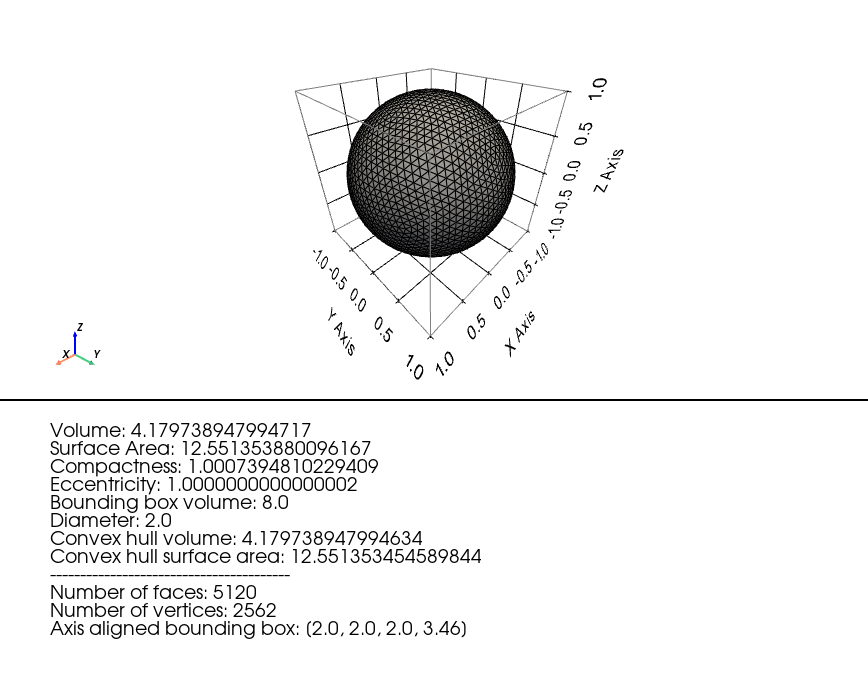
\includegraphics[width=\textwidth]{assets/feature_extraction/scalar_features/sphere.png}
    \caption{Sphere scalar features}
    \label{fig:sphere-scalars}    
    \end{subfigure}
    \hfill
    \begin{subfigure}[b]{0.45\textwidth}
        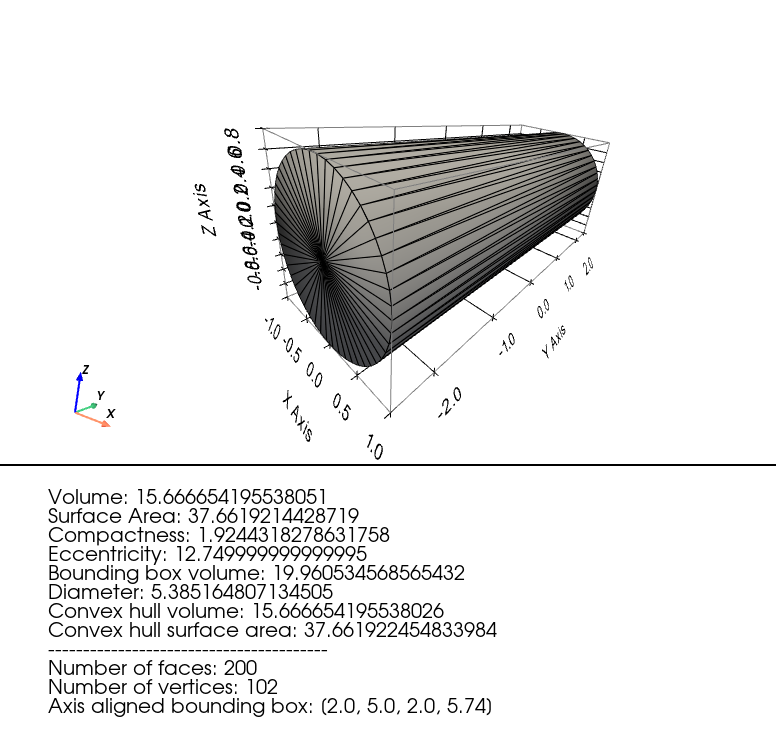
\includegraphics[width=\textwidth]{assets/feature_extraction/scalar_features/cylinder.png}
    \caption{Cylinder scalar features}
    \label{fig:cylinder-scalars}
    \end{subfigure}
    \hfill
    
    \begin{subfigure}[b]{0.45\textwidth}
        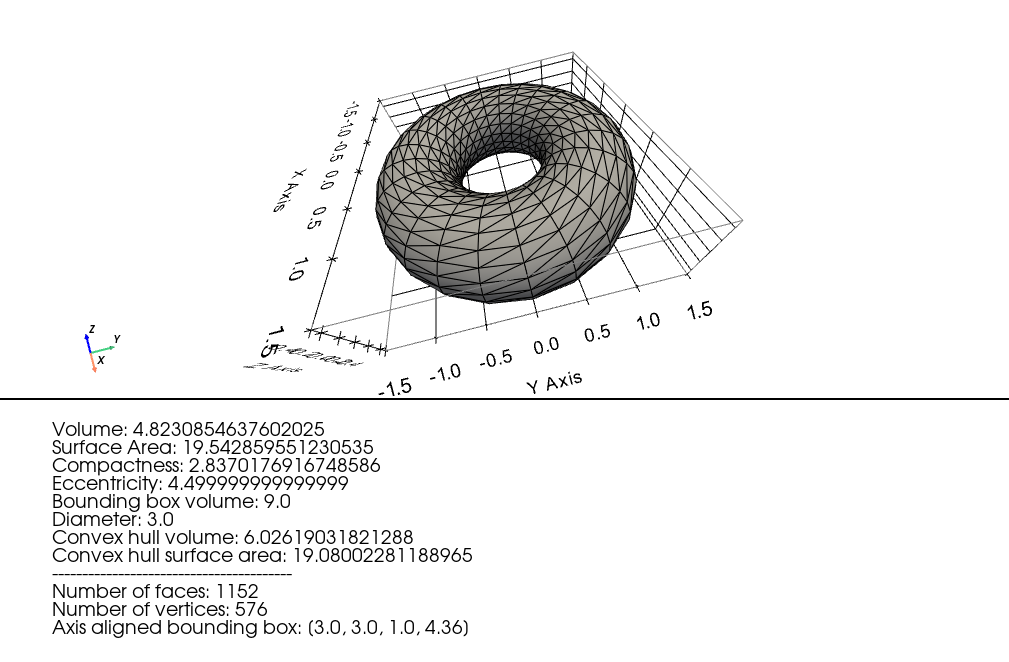
\includegraphics[width=\textwidth]{assets/feature_extraction/scalar_features/torus.png}
    \caption{Torus scalar features}
    \label{fig:torus-scalars}   
    \end{subfigure}

    \caption{Global descriptors for several 3D shapes}
    \label{fig:global-descriptors-proof} 
\end{figure}


\begin{figure}[ht!p]
    \centering
    \begin{subfigure}[b]{0.45\textwidth}
        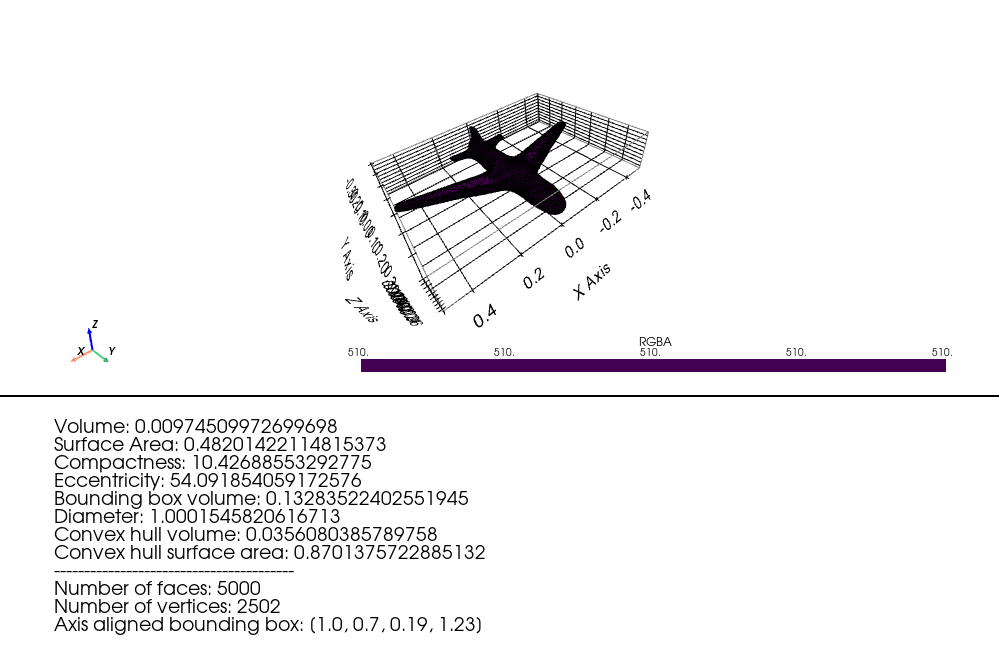
\includegraphics[width=\textwidth]{assets/feature_extraction/scalar_features/airplane.png}
        \caption{Airplane}
        \label{fig:airplane-scalars}
    \end{subfigure}
    \hfill
    \begin{subfigure}[b]{0.45\textwidth}
        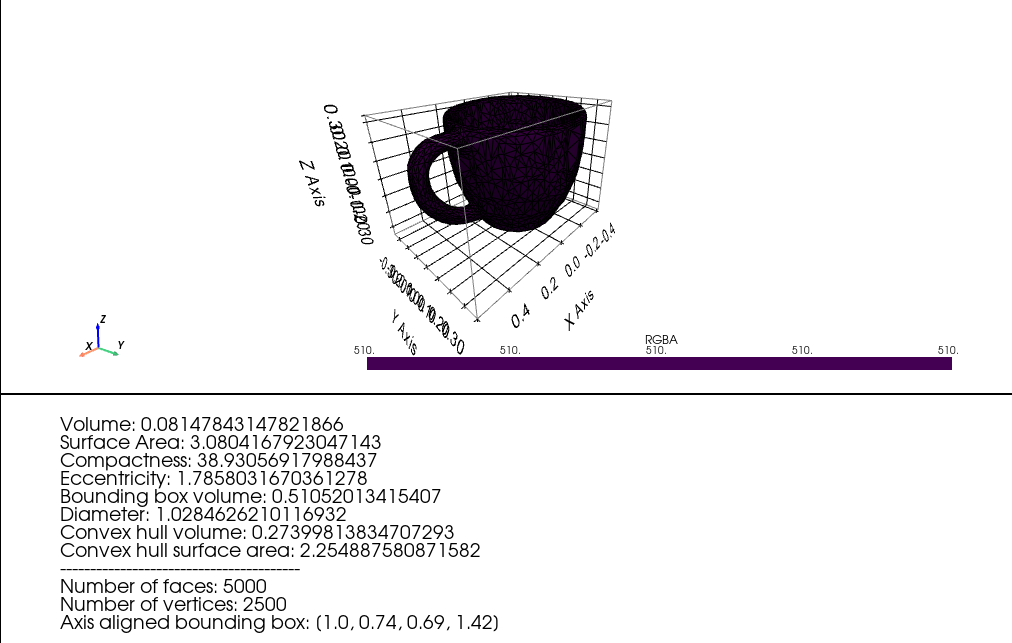
\includegraphics[width=\textwidth]{assets/feature_extraction/scalar_features/cup.png}
        \caption{Cup}
        \label{fig:cup-scalars}
    \end{subfigure}
    \hfill
    
    \begin{subfigure}[b]{0.45\textwidth}
        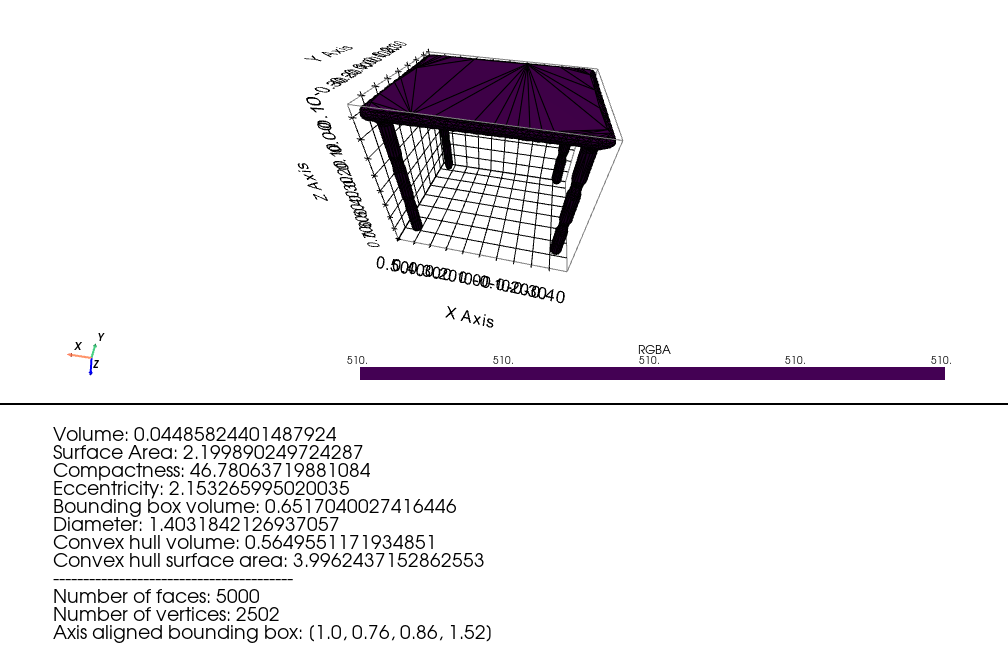
\includegraphics[width=\textwidth]{assets/feature_extraction/scalar_features/table.png}
        \caption{Table}
        \label{fig:table-scalars}
    \end{subfigure}
    \hfill
    \begin{subfigure}[b]{0.45\textwidth}
        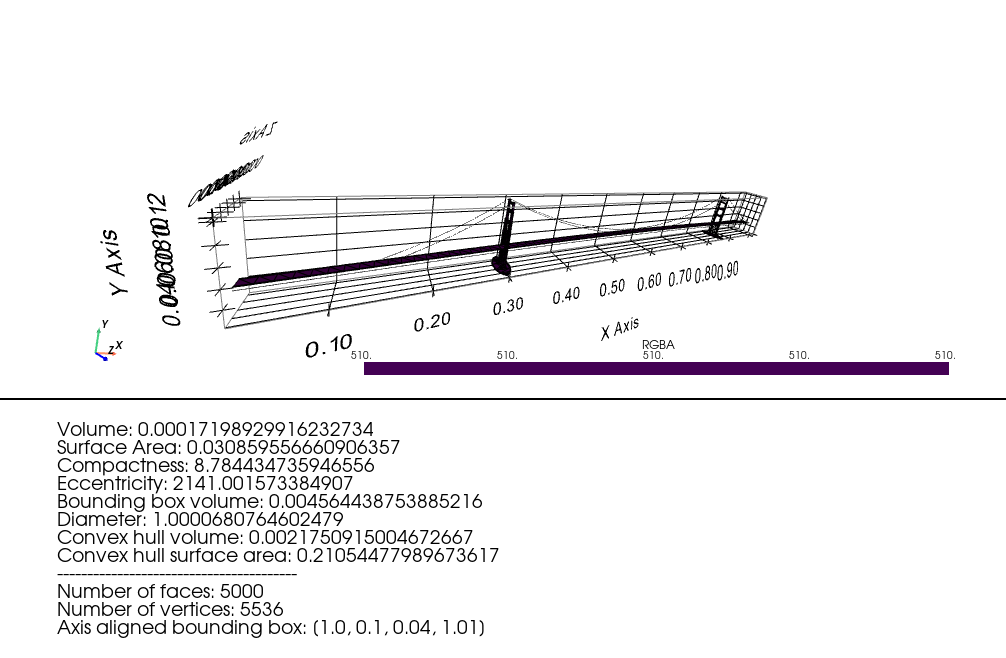
\includegraphics[width=\textwidth]{assets/feature_extraction/scalar_features/bridge.png}
        \caption{Bridge}
        \label{fig:bridge-scalars}
    \end{subfigure}
    \caption{Global descriptors for 3D shapes from our data set}
    \label{fig:global-descriptors-dataset}
\end{figure}